\documentclass[11pt]{beamer}
\beamertemplatenavigationsymbolsempty
\setbeamertemplate{footline}[frame number]

\makeatletter
\newlength\beamerleftmargin
\setlength\beamerleftmargin{\Gm@lmargin}
\makeatother


\usepackage[utf8]{inputenc}
\usepackage[english]{babel}
\usepackage[absolute,overlay]{textpos}
\usepackage{amsmath}
\usepackage{amsfonts}
\usepackage{amssymb}
\usepackage{graphicx}
\usepackage{multirow}
\usepackage{pbox}
\usepackage{array}

\usetheme{Warsaw}

\newcommand{\norm}[1]{\left\lVert#1\right\rVert}
\newcommand{\normsq}[1]{\left\lVert#1\right\rVert^2}
\setbeamercolor{framesource}{fg=gray}
\setbeamerfont{framesource}{size=\tiny}

\newcommand{\MX}{\mathbf{X}} %uncentered data
\newcommand{\MC}{\mathbf{C}} %centering
\newcommand{\MY}{\mathbf{Y}} %centered data
\newcommand{\MF}{\mathbf{F}_2} %F2-distance matrix
\newcommand{\MFT}{\mathbf{F}_3} %F3-distance matrix
\newcommand{\MP}{\mathbf{P}} % PCs
\newcommand{\ML}{\mathbf{L}} % loadings
\newcommand{\MK}{\mathbf{K}} % Kernel
\newcommand{\MSINGULAR}{\mathbf{\Sigma}} % Singular values matrix
\newcommand{\MEIGEN}{\mathbf{\Lambda}} % Eigenvalue matrix

\newcommand{\MEAN}{\boldsymbol{\mu}} % Kernel

\newcommand{\POP}[1]{X_{#1}}
\newcommand{\POPX}{\POP{X}}
\newcommand{\POPA}{\POP{A}}
\newcommand{\POPO}{\POP{O}}
\newcommand{\q}[1]{\hat{p}_{#1}}
\newcommand{\HAP}[1]{I_{#1}}
\newcommand{\HET}[1]{H_{#1}}
%\newcommand{\PCOAL}[2]{c_{#1\downarrow #2}}
\newcommand{\PCOAL}[2]{f}
\newcommand{\FX}[1]{F_{#1}}



\newcommand{\source}[1]{\begin{textblock*}{4cm}(8.7cm,8.6cm)
		\begin{beamercolorbox}[ht=0.5cm,right]{framesource}
			\usebeamerfont{framesource}\usebeamercolor[fg]{framesource} {#1}
		\end{beamercolorbox}
\end{textblock*}}


\begin{document}
	\author{Benjamin Peter}
	\title{F-statistics and PCA}
	%\subtitle{}
	%\logo{}
	%\institute{}
	%\date{}
	%\subject{}
	%\setbeamercovered{transparent}
	%\setbeamertemplate{navigation symbols}{}
	\begin{frame}[plain]
	\maketitle
\end{frame}

\begin{frame}
\frametitle{Population structure and ancient DNA}
\begin{center}
		\hspace*{-1.8\beamerleftmargin}
		\includegraphics<1>[width=\textwidth]{data/figures/ancient_dna_by_year.png}
		\includegraphics<2>[width=1.05\paperwidth]{data/figures/ancient_dna_map.png}		
\end{center}
		 \source{\url{https://reich.hms.harvard.edu/}}
\end{frame}

\begin{frame}
\frametitle{PCA and $F$-statistics}
\begin{columns}
	\begin{column}{0.5\textwidth}
		\includegraphics[width=1.8\textwidth]{figures/hajdinjak2021_fig2a.png}
	\end{column}
	\begin{column}{0.5\textwidth}
		\includegraphics[width=1.5\textwidth]{figures/hajdinjak2021_fige2.png}
		\source{Hajdinjak et al. 2021}
	\end{column}
\end{columns}
\end{frame}
\begin{frame}
\frametitle{Goals of this talk}
\begin{itemize}
	\item Technical \& Conceptual Background
	\item Establish conceptual links between frameworks
	\begin{enumerate}
		\item How can we interpret PCA in context of $F$-stats?
		\item How can we interpret $F$-stats in the context of PCA?		
	\end{enumerate}
	\item (Use established links to improve data interpretation)
\end{itemize}
\only<2>{
\begin{alertblock}{Focus on intuition}
	Some details in terms of estimation, normalization, missing data will be glossed over
\end{alertblock}
}
\end{frame}


\begin{frame}
\frametitle{$F$-statistics}
  \begin{tabular} {m{8.5cm}  |m{2cm}  }
	Definition & Branch length \\%& Path  \\
	\hline
	\vspace{6pt}$$\FX2(\POP1,\POP2) = \sum_l (X_{il} - X_{jl})^2 - H_1 - H_2$$
	&\vspace{6pt}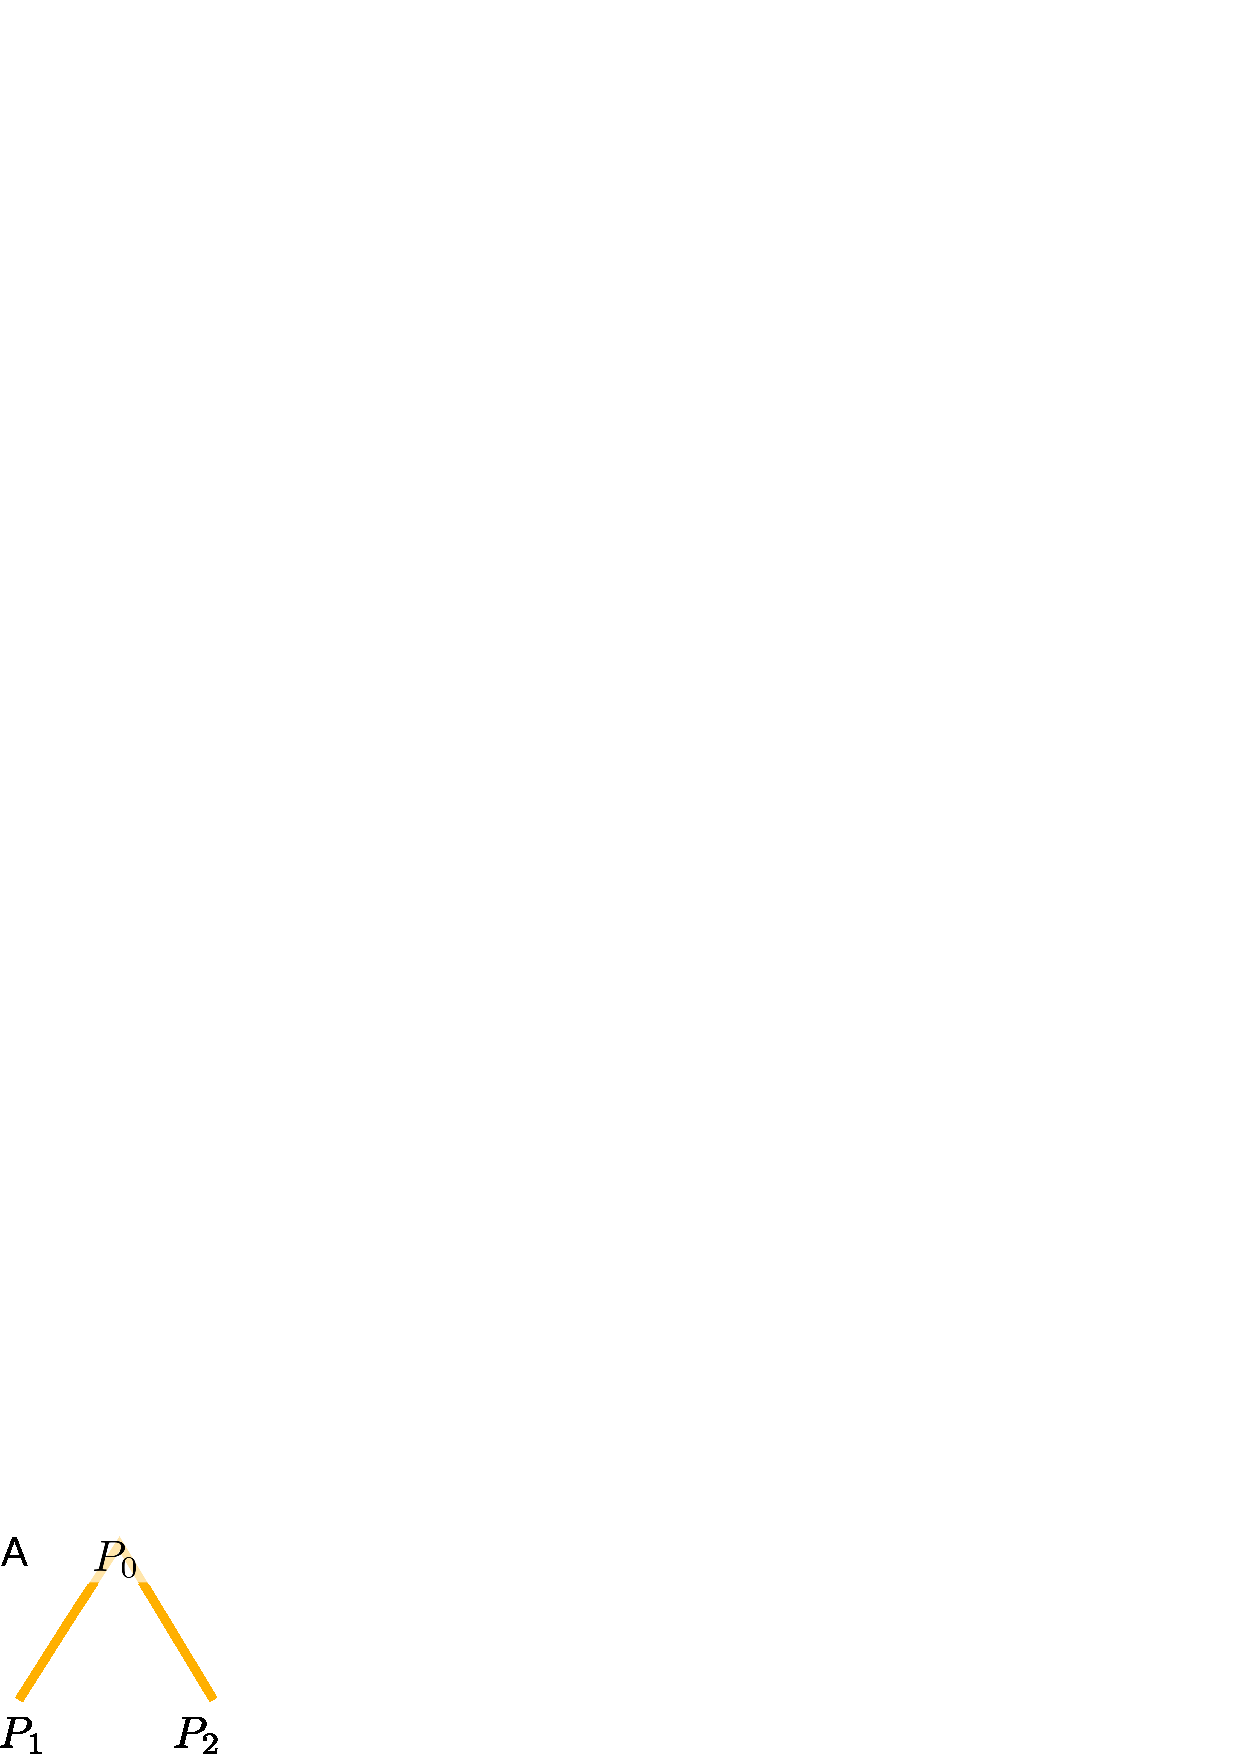
\includegraphics[scale=0.4]{figures/f2_internal.pdf}        
	%&\vspace{6pt}\includegraphics[scale=0.5]{./f2_admixture.eps}        
	\\ 
	\hline
	\only<2->{
	$$\FX3(\POP{x}; \POP1, \POP2) = \sum_l(X_{xl} - X_{1l})(X_{xl} - X_{2l}) - H_X$$
     $$\FX3(X_x; X_1, X_2) = F_2(X_x, X_1) + F_2(X_x, X_2) - F_2(X_1, X_2)$$
	&\vspace{6pt}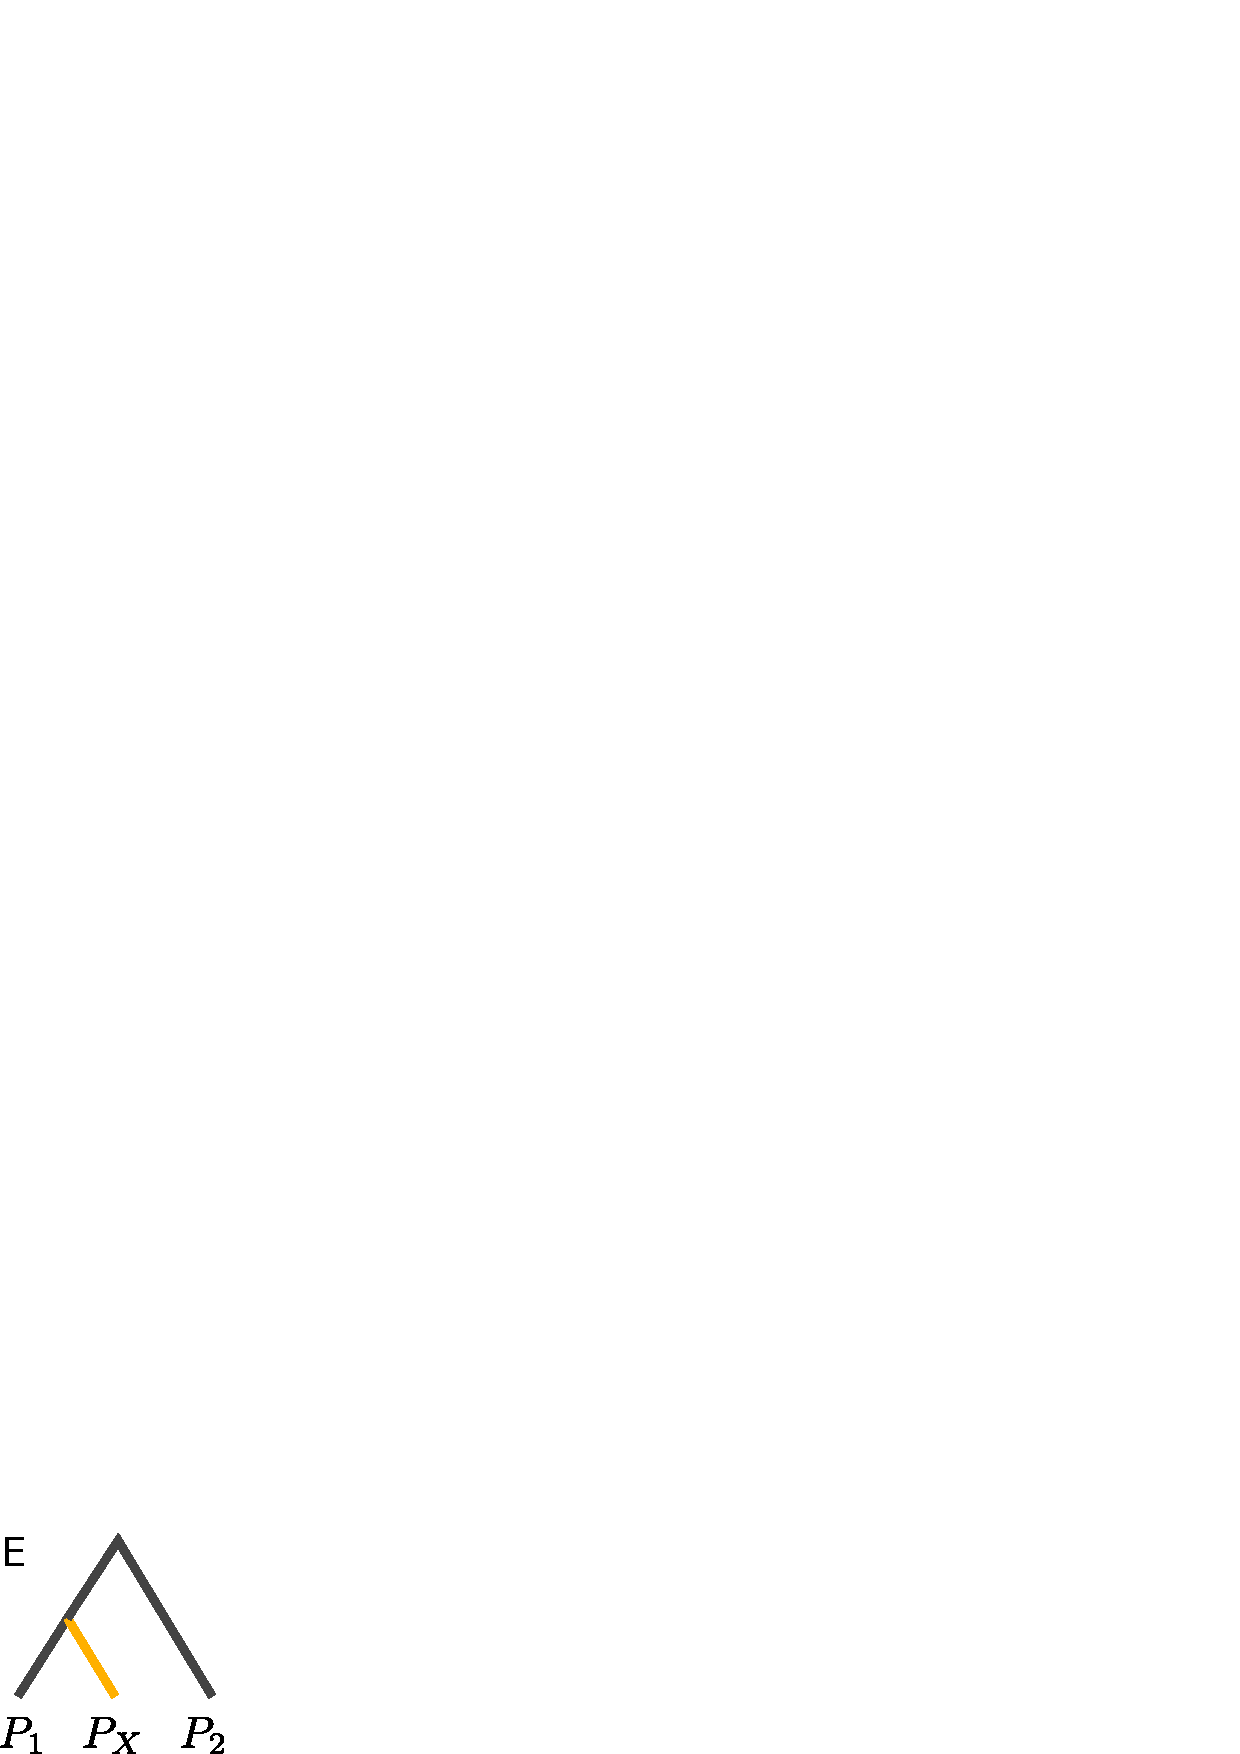
\includegraphics[scale=0.4]{figures//f3_internal.pdf}        
	%&\vspace{6pt}\includegraphics[scale=0.5]{./f3_admixture.eps}        
	\\ 
	\hline}
\only<3>{``Admixture''-$F_3$-statistic: If data is generated by a tree-like relationship, $F_3(P_X; P_1, P_2) \geq 0$
	&\vspace{6pt}\includegraphics[scale=0.4]{figures//f3_admixture.pdf}      
	\\ 
	\hline
}
\only<4>{``Outgroup''-$F_3$-statistic: Most similar pops have highest $F_3(P_2; P_X, P_1)$
	&\vspace{6pt}\includegraphics[scale=0.4]{figures//f3_outgroup.pdf}      
	\\ 
	\hline
}
	\only<5>{$$\FX4^{(B)}(\POP1; \POP2; \POP3, \POP4) = \sum_l(X_{1l} - X_{3l})(X_{2l} - X_{4l})$$
	&\vspace{6pt}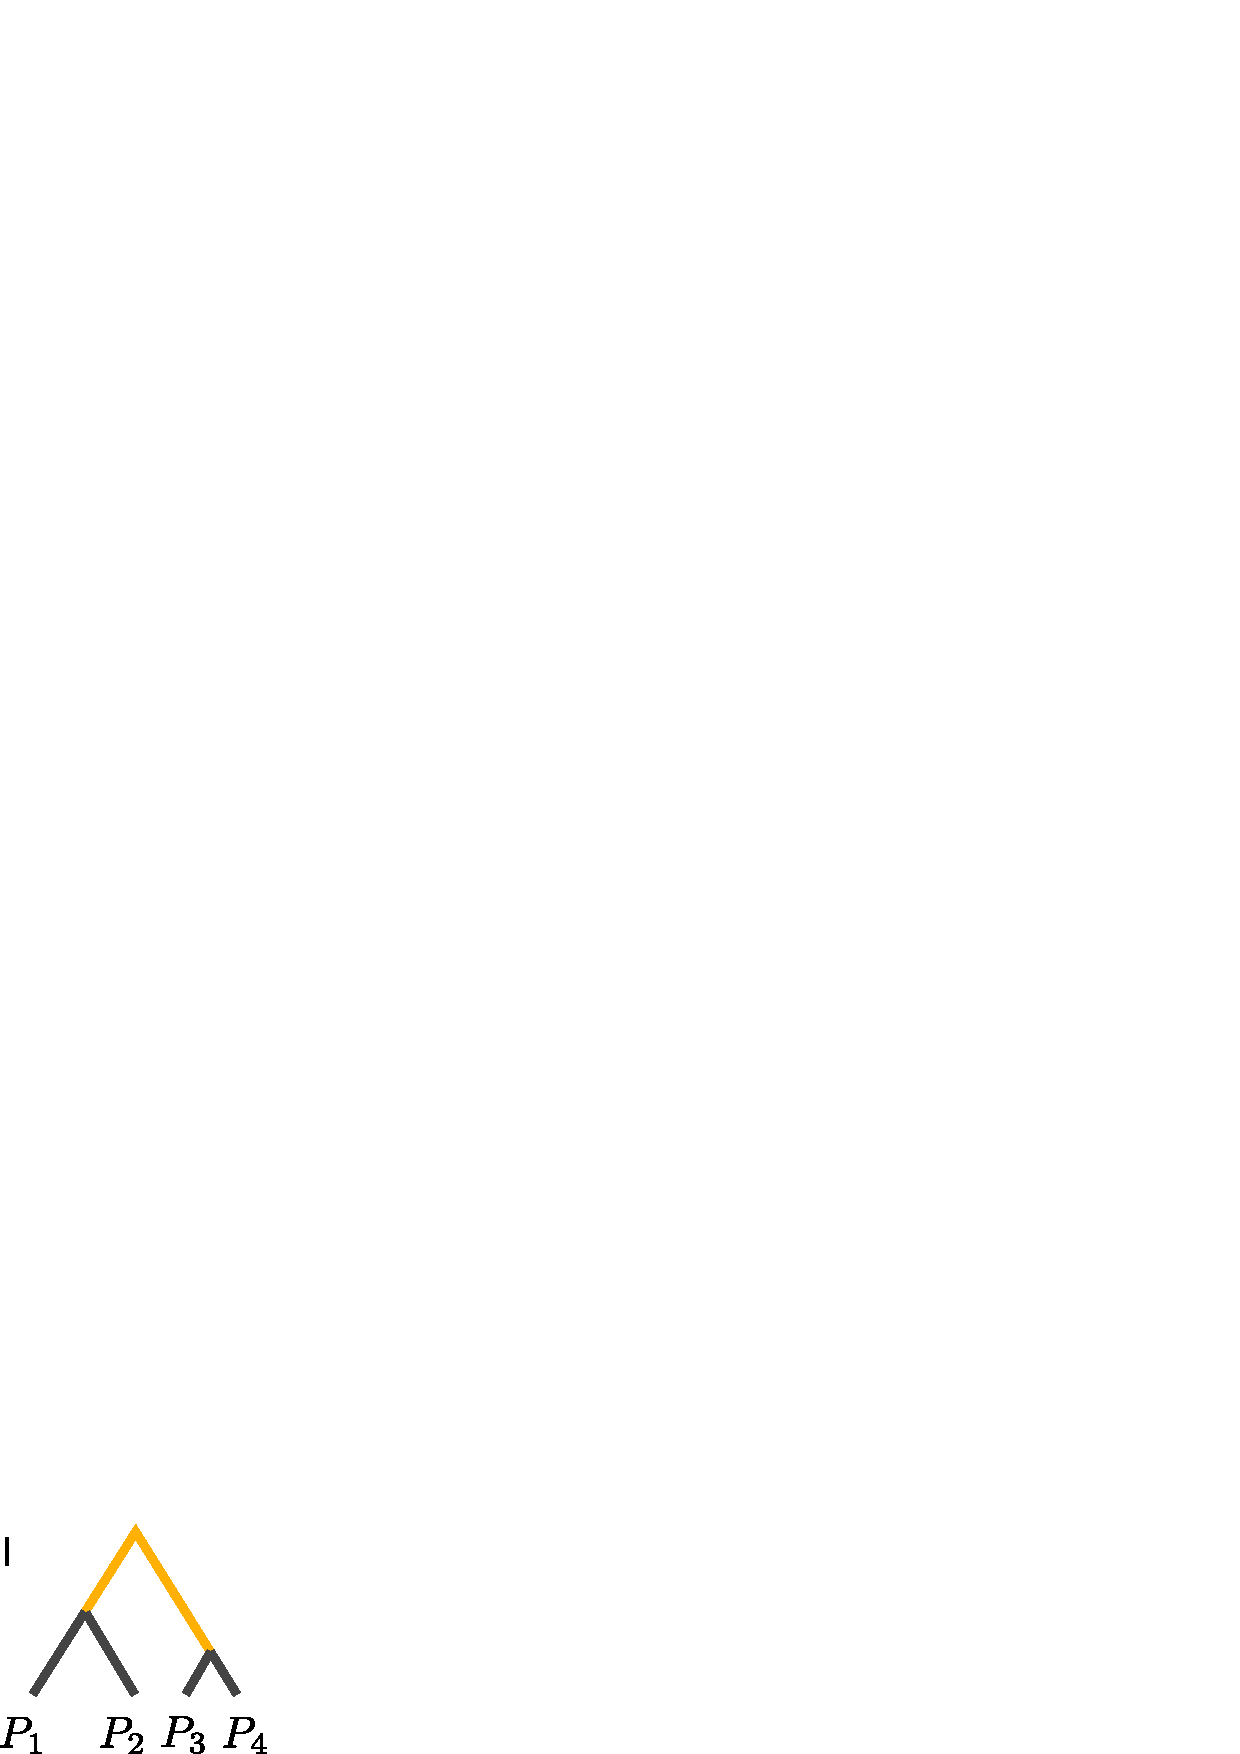
\includegraphics[scale=0.4]{figures//f4_internal_branch.pdf}        
	%&\vspace{6pt}\includegraphics[scale=0.5]{./f4b_admixture.pdf}        
	\\ 
	\hline
	}
	\only<6>{
	$$\FX4^{(T)}(\POP1; \POP2; \POP3, \POP4) = = \sum_l(X_{1l} - X_{2l})(X_{3l} - X_{4l})$$
	&\vspace{6pt}\includegraphics[scale=0.4]{figures//f4_internal.pdf}        
	%&\vspace{6pt}\includegraphics[scale=0.5]{./f4_admixture.eps} \\ 
}
\end{tabular}

		\source{Patterson et al. 2012; Peter 2016}

\end{frame}



\begin{frame}
\frametitle{Principal Component Analysis}
\begin{columns}
	\begin{column}{0.5\textwidth}
		\includegraphics[width=1.5\textwidth]{figures/hajdinjak2021_fige2.png}
	\end{column}
	\begin{column}{0.5\textwidth}
		\includegraphics<2>[width=1\textwidth]{figures/mcvean2009_fig3ab.png}		
		\includegraphics<2>[width=1\textwidth]{figures/mcvean2009_fig4b.png}
		\source{McVean, 2009}
	\end{column}
\end{columns}
\end{frame}
	\begin{frame}
\frametitle{Principal Component Analysis}
\begin{columns}
	\begin{column}{0.5\textwidth}
		\includegraphics<1>{figures/pca1.pdf}
		\includegraphics<2>{figures/pca2.pdf}
		\includegraphics<3>{figures/pca3.pdf}
		\includegraphics<4>{figures/pca4.pdf}
		\includegraphics<5>{figures/pca5.pdf}						
		\includegraphics<6>{figures/pca6.pdf}								
	\end{column}
	\begin{column}{0.5\textwidth}
		\begin{itemize}
			\item<1-> Raw SNP data $\MX; x_{ij}$
			\item<2-> Centering $\MY = \MC\MX; y_{ij}= x_{ij} - \mu_j$
			\only<3>{\item<3> Rotation $\MY = \underbrace{\MP}_\text{PCs}\underbrace{\ML}_\text{Rotation}$}
			\item<4-> Rotation $\MY = \MP\ML$		
			\item<5-> Truncation $\hat{\MP} = \begin{pmatrix}
			\mathbf{p}_1\\
			\mathbf{p}_2\\		
			\hline\\
			\vdots\\
			\mathbf{p}_n\\		
			\end{pmatrix} $		
			\item<6-> Approximation $\hat{\MY} = \hat{\MP}\hat{\ML}		$
			
		\end{itemize}
		
	\end{column}
\end{columns}
\end{frame}



\begin{frame}
\frametitle{How to find PCs}
\begin{columns}
\begin{column}{0.4\textwidth}
	\includegraphics[width=\textwidth]{figures/pca3.pdf}
\end{column}
\begin{column}{0.6\textwidth}
	\begin{itemize}
		\item<1-> Singular Value Decomposition: $\MY = (\mathbf{U}\mathbf{D})\mathbf{L} = \mathbf{P}\mathbf{L}$
		\item<2-> Eigendecomposition of $\MY\MY^T$: $\MY\MY^T = \mathbf{U}\mathbf{D}^2\mathbf{U}^T = \MP\MP^T$
		\only<3>{\item $y_{ij}$}
		\item<4-> $y_{ij} = \sum_l (x_{il} - \mu_l)(x_{jl} - \mu_l)$
		\item<5-> $y_{ij} = F_3(\MEAN; \MX_i, \MX_j)$
	\end{itemize}
\end{column}			
\end{columns}
\vspace{30px}
\only<6>{
\begin{alertblock}{Observation}
	PCA is equivalent to outgroup-$F_3$-analysis with sample mean as outgroup
\end{alertblock}
}
\end{frame}


\begin{frame}
\frametitle{(metric) Multi-Dimensional Scaling (MDS)}

\begin{columns}
\begin{column}{0.5\textwidth}
\includegraphics<1>{figures/pca1.pdf}
\includegraphics<2>{figures/mds1.pdf}
\includegraphics<3->{figures/mds2.pdf}
\end{column}
\begin{column}{0.5\textwidth}
\includegraphics<4>{figures/mds3.pdf}		
\includegraphics<5>{figures/mds4.pdf}		
\includegraphics<6>{figures/mds5.pdf}		
\includegraphics<7>{figures/mds6.pdf}					
\end{column}
\end{columns}
\end{frame}


\begin{frame}
\frametitle{PCA is MDS on $\MF$}

\begin{itemize}
\item<1-> PCA is decomposition of Covariance matrix: $\MY\MY^T$
\item<2-> Consider $\MF; f_{ij} = F_2(X_i, X_j) = X_i^2 + X_j^2 - 2 X_i X_j$
\item<3-> MDS is Eigendecomposition of $-\frac{1}{2}\MC\MF\MC$
\item<4-> $\MC\MF\MC = \underbrace{\MC\MX_i^2\MC}_{0}  + \underbrace{\MC\MX_i^2\MC}_{0} - 2\underbrace{\MC\MX\MX^T\MC}_{\MY\MY^T}$
\end{itemize}


\only<5>{
\begin{alertblock}{Observation}
PCA is equivalent to MDS on $\MF$
\end{alertblock}
}
\end{frame}

\begin{frame}
\frametitle{PCA is MDS on Outgroup$\MFT$}

\begin{itemize}
\item<1-> PCA is decomposition of Covariance matrix: $\MY\MY^T$
\item<2-> Consider $\MFT(O); f_{ij} = F_3(O; X_i, X_j) = O^2 - OX_i - OX_j +  X_i X_j$
\item<4-> $\MC\MFT\MC = \underbrace{\MC O^2\MC}_{0}  - 
\underbrace{\MC O\MX_i\MC}_{0} -
\underbrace{\MC O\MX_j\MC}_{0} + 
\underbrace{\MC\MX\MX^T\MC}_{\MY\MY^T}$
\end{itemize}


\only<5>{
\begin{alertblock}{Observation}
Decomposition of \emph{any} centered $F_3$-matrix is equivalent to PCA.
\end{alertblock}
}
\end{frame}


\begin{frame}
\frametitle{0-diagonal MDS}
\end{frame}


\begin{frame}
\frametitle{$F$-statistics on PCA-plot}
\begin{itemize}
	\item Recall that PCA is just translation + rotation
	\item<2-> Distances (such as $F_2$) are invariant to translation + rotation
	\item<3-> $$F_2(X_1, X_2) = \sum_{\text{loci}}(x_{1l} - x_{2l})^2$$
	\item<4-> $$F_2(X_1, X_2) = \sum_{\text{PCs}}(x_{1p} - x_{2p})^2$$	
\end{itemize}
\only<5->{
	\begin{alertblock}{Observation}
		$F_2$ can be decomposed in contributions of different principal components
	\end{alertblock}
}
\end{frame}


\begin{frame}
\frametitle{$F$-statistics on PCA-plot}
\begin{columns}
	\begin{column}{0.5\textwidth}
		\includegraphics<1>{figures/pca1.pdf}
		\includegraphics<2->{figures/pca1b.pdf}		
	\end{column}
	\begin{column}{0.5\textwidth}
		\begin{itemize}
			\item<3-> $F$-statistics have a geometrical representation on PCA-plot
			\item<3-> Exact only if we use \emph{all} PCs
			\item<4-> Good approximation for 2D-plot if first 2 PCs capture relevant population structure
		\end{itemize}		
	\end{column}
\end{columns}
\end{frame}

\begin{frame}
\frametitle{$F_2$-statistic on PCA-plot}
\begin{columns}
	\begin{column}{0.5\textwidth}
		\includegraphics{figures/f2_on_pca.pdf}
	\end{column}
	\begin{column}{0.5\textwidth}
		\begin{itemize}
			\item $F_2(X_1, X_2) = \sum_l(X_{1l}-X_{2l})^2$
			\item $F_2(X_1, X_2) = \normsq{X_1, X_2}$			
		\end{itemize}		
	\end{column}
\end{columns}
\end{frame}

\begin{frame}
\frametitle{Admixed populations ($F_3$) on PCA-plot}
\begin{columns}
	\begin{column}{0.4\textwidth}
		\includegraphics<1>{figures/f3_on_pca_1b.pdf}
		\includegraphics<2-4>{figures/f3_on_pca_1.pdf}		
		\includegraphics<5>{figures/f3_on_pca_1c.pdf}				
	\end{column}
	\begin{column}{0.6\textwidth}
		\begin{itemize}
			\item<1-> Given $X_1, X_2$, which pops have $F_3 < 0$?	
			\item<2-> $F_3(Y; X_1, X_2) = 0$ is a circle!
%			\item<3-> Samples outside circle will always have positive $F_3$
			\item<5> $F_3(Y; X_1, X_2) = k < 0$ is smaller circle
		\end{itemize}		
		\includegraphics<4>[width=\textwidth]{figures/mcvean2009_fig4b.png}\source{McVean 2009}
	\end{column}
\end{columns}
\end{frame}





\begin{frame}
\frametitle{Admixture $F_3$-stats on PCA-plot}
\begin{columns}
	\begin{column}{0.4\textwidth}
		\includegraphics<1>{figures/f3_on_pca_2b.pdf}
		\includegraphics<2->{figures/f3_on_pca_2.pdf}		
	\end{column}
	\begin{column}{0.6\textwidth}
		\begin{itemize}
			\item<1-> Given $X_1, X_x$, which pops $X_2$ have $F_3 < 0$?	
			\item<2-> $F_3$ is 0 if $(X_x; X_1), (X_x; X_2)$ form a right angle!
			\item<3-> Inner (dot) product: $F_3(X_x; X_1, X_2) = \langle X_x - X_1, X_x - X_2\rangle$
		\end{itemize}		
	\end{column}
\end{columns}
\end{frame}


\begin{frame}
\frametitle{ $F_4$-stats on PCA-plot}
\begin{columns}
	\begin{column}{0.4\textwidth}
		\includegraphics{figures/f4_on_pca.pdf}
	\end{column}
	\begin{column}{0.6\textwidth}
		\begin{itemize}
			\item<1-> $F_4$ is projection of $\overline{X_3X_4}$ on $\overline{X_1X_2}$
%			\item<2-> $F_4$ is zero if $\overline{X_3X_4}$ and $\overline{X_1X_2}$ are orthogonal
		\end{itemize}		
	\end{column}
\end{columns}
\end{frame}

\begin{frame}
\frametitle{Where does Orthogonality come from?}
\begin{columns}
	\begin{column}{0.5\textwidth}
		\includegraphics{figures/f3_nonorthogonal.pdf}
	\end{column}
	\begin{column}{0.5\textwidth}
		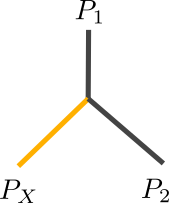
\includegraphics{figures/f3_orthogonal.pdf}
	\end{column}
\end{columns}
\end{frame}

\begin{frame}
\frametitle{Applications}
\begin{enumerate}
	\item <1->Better link $F$-stats and PCA results
		\begin{itemize}
			\item<1-> use Dimensions / Orthogonality for useful data representations
		\end{itemize}	
 	\item<2-> Distinguish admixture events
\begin{itemize}
	\item<3-> same $F_3$ value may arise from distinct admixture events, PCs may point to differences
\end{itemize}
\item<4-> Understand discrepancies
\begin{itemize}
	\item<4-> most likely due to data artifacts / higher PCs
\end{itemize}	
	\item <5->Standardize normalization 
	\begin{itemize}
		\item <5->$F_2^{(\text{PCA})} = \frac{1}{\hat\sigma}\sum(X_i - X_j)^2$
		\item <5->$F_2^{(\text{F-stats})} = \sum(X_i - X_j)^2$		
	\end{itemize}
%    \item<6-> Model populations where gene flow is common
%		\begin{itemize}
%			\item<6-> $F$-statistics assume gene flow is rare
%		\end{itemize}
    \item<7-> Better out-of-sample predictions
\begin{itemize}
	\item<7-> \texttt{qpGraph} and other tools fail with large samples
\end{itemize}
    
\end{enumerate}
\end{frame}




\end{document}